\documentclass[a4paper,10pt]{article}

%\usepackage[utf8]{inputenc}
\usepackage{graphicx}
\usepackage{url}
\usepackage{float}
\usepackage{times}
\usepackage{multirow}
\usepackage{listings}
\usepackage{times}
\usepackage{paralist}
\usepackage{epsfig}
\usepackage{subfigure}
\usepackage[hypertex]{hyperref}
\usepackage{subfigure}
\usepackage{color}
\usepackage{ifpdf}

\newcommand{\I}[1]{\textit{#1}}
\newcommand{\B}[1]{\textbf{#1}}
\newcommand{\BI}[1]{\textbf{\textit{#1}}}
\newcommand{\T}[1]{\texttt{#1}}
\newcommand{\dctf}{dC$_{25}$ }
\newcommand{\dctfnsp}{dC$_{25}$}
\newcommand{\atf}{A$_{25}$ }
\newcommand{\dco}{dC$_{1}$ }
\newcommand{\atfnsp}{A$_{25}$}
\newcommand{\dconsp}{dC$_{1}$}
\newcommand{\aonsp}{A$_{1}$}
\newcommand{\ao}{A$_{1}$ }
\newcommand{\ato}{A$_{1}$ }
\newcommand{\ahl}{$\alpha$HL }
\newcommand{\ahlnsp}{$\alpha$HL}
\newcommand{\prim}{$^{\prime}$ }
\newcommand{\primnsp}{$^{\prime}$}


\pdfpagewidth 8.5in
\pdfpageheight 11in 

\setlength\topmargin{0in}
\setlength\headheight{0in}
\setlength\headsep{0in}
\setlength\textheight{9in}
\setlength\textwidth{6.5in}
\setlength\oddsidemargin{0in}
\setlength\evensidemargin{0in}
\setlength\parindent{0.1in}
\setlength\parskip{0.25em}

\ifpdf
 \DeclareGraphicsExtensions{.pdf, .jpg, .png}
\else
 \DeclareGraphicsExtensions{.eps, .ps}
\fi

\newcommand{\jha}[1]{ {\textcolor{red} { ***Jha: #1 }}}

\begin{document}
\title{\large % Investigating Scale-Out Performance of 
% Loosely-Coupled Simulations Using Multiple Distributed Resources on the TeraGrid.
  We need an appropriate Title}

\author{Principal Investigator: Shantenu Jha$^{1,2}$ \\
Co-Principal Investigator: Joohyun Kim$^{1}$ \\ 
Co-Principal Investigator: Yaakoub El Khamra$^{3}$\\\
   \small{\emph{$^{1}$Center for Computation \& Technology, Louisiana State University, Baton Rouge, 
USA}}
\\
  \small{\emph{$^{2}$Department of Computer Science, Louisiana State
      University, Baton Rouge, USA}}
\\
  \small{\emph{$^{3}$Texas Advanced Computing Center TACC, University of Texas, Austin, USA}}}

\newif\ifdraft
\drafttrue
\ifdraft
\newcommand{\amnote}[1]{ {\textcolor{magenta} { ***AM: #1c }}}
\newcommand{\jhanote}[1]{ {\textcolor{red} { ***SJ: #1 }}}
\newcommand{\michaelnote}[1]{ {\textcolor{blue} { ***MM: #1 }}}
\else
\newcommand{\amnote}[1]{}
\newcommand{\jhanote}[1]{}
\newcommand{\michaelnote}[1]{ {\textcolor{blue} { ***MM: #1 }}}
\fi


\date{15 July 2010}

\maketitle

\subsection*{Summary:} 

We propose to use multiple TeraGrid resources both in concurrent usage mode, as well as individual resources to study several scientific problems.  

This work is built on the extensive efforts over the past two years we have carried out with a wide range of computational science and computer science projects, requiring a few groups to use multiple resources on the TeraGrid concurrently (for loosely-coupled simulations).  

Specifically, in this proposal we request XXXXM SUs for four distinct projects: (i) understanding translocation of nucleic acid in $\alpha$-Hemolysin protein pores; (ii) elucidating the conformational switching of S-box riboswitches, (iii) UCL project and, (iv) developing and enhancing the understanding of distributed applications and testing the {\it scale-out } performance of a range of applications. The projects for which resources are being requested are all funded projects -- mostly at the National/International level, and some by local resources. Project 2 which is not currently funded by Federal/National agencies is the basis for upcoming significant proposals.  Additionally, the request for XXXXM SUs in this proposal is based upon the projected science problems as outlined below as well as a proven track record of {\it successfully} utilising more than YYYYM SUs in the \jhanote{number of years}.

% \jhanote{Yaakoub, please determine the correct units?  Is it SUs, NU or some other metric. Thanks.}

% \jhanote{Issues: Final Number of CPU Hrs?  Which resource? What component should be roaming?}

\section{Results From Prior Awards}

\jhanote{This should list out (i) prior awards and what they were for, (ii) scientific progress and understanding that arose and (ii) publications as a result of prior awards.}

\section{Project 1: Nucleic Acid Translocation through Alpha-Hemolysic Protein Nanopore}

The translocation of polynucleotides across membranes is a fundamental biological process, with important technological and medical relevance.  The translocation process is complex and is influenced by a range of factors including the diameter and inner surface of the pore, the secondary structure of the polymer, and interactions between polymer and protein. We have performed non-equilibrium constant velocity-steered molecular dynamics (cv-SMD) simulations of nucleic acid molecule translocation through the protein nanopore $\alpha$-hemolysin (\ref{fig:edge}) and used Jarzynski's identity~\cite{jarz} to determine the associated free energy profiles. Constant velocity-steered molecular dynamics~\cite{namd} (cv-SMD) is a type of non-equilibrium simulation that connects an atom or center of mass of a group of atoms via a harmonic spring (governed by a force or spring constant, $k$) to a constraint position which is moved at constant velocity. Cv-SMD has the advantage of a well defined wall-clock and simulated time-frame for a given translocation distance, allowing the induction of high-speed translocation in a consistent manner.

\begin{figure}[!h]
  \begin{center}
    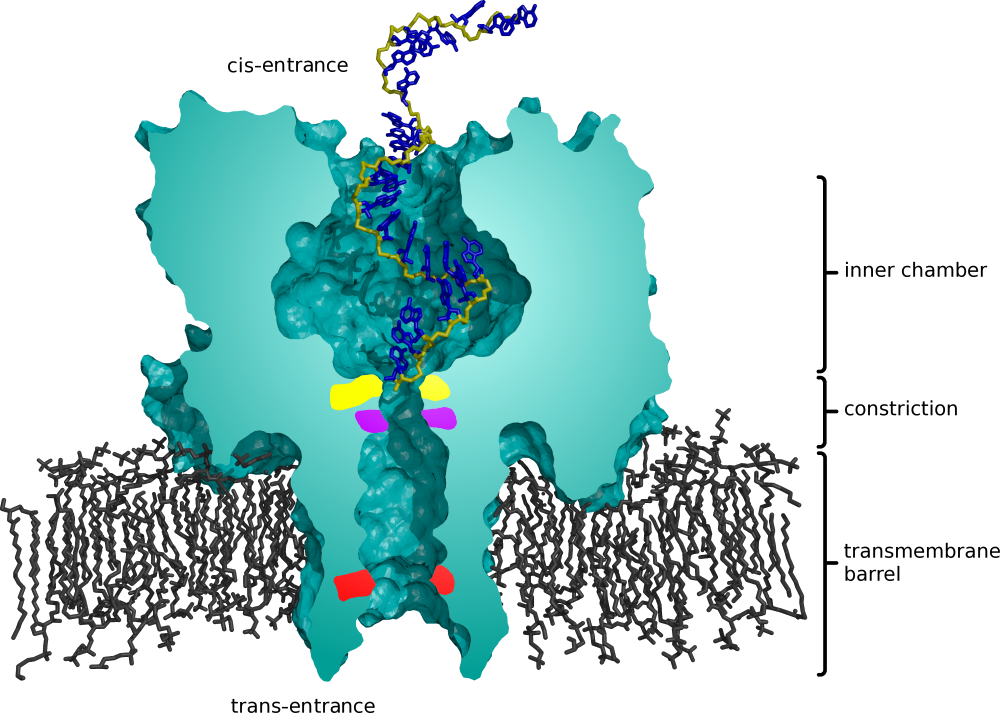
\includegraphics[width=5.0in]{ahl_labelled13}
  \end{center}
  \caption{Figure from JCTC Publication, representing the starting configuration of a 3\prim led \atf translocation simulation. The heptameric protein pore \ahl (green) is inserted into a lipid bilayer (black). Features of the translocating molecule include the backbone of \atf (dark yellow) and the nucleic acid bases (blue). The $trans$-entrance is at the bottom of the pore; taking the $trans$-entrance of \ahl as a reference point at 0~{\AA}, other notable features include protein residue Leu-135 at 13~{\AA} (red), Met-113 at 43~{\AA} (pink), Lys-147 at 45~{\AA} (light yellow), and the $cis$-entrance at the top of the protein at 95~{\AA}. The $cis$-entrance is 28~{\AA} in diameter, the wide section of the pore running from the $cis$-entrance to residue Lys-147 is termed the inner chamber and is up to 46~{\AA} wide. The constriction marked by residues Lys-147 and Met-113 is 14~{\AA} wide, while the transmembrane barrel runs from the constriction to the $trans$-entrance and is around 20~{\AA} wide; the $trans$-entrance is 24~{\AA} wide. The C3\prim carbon atom of the 3\prim end residue of \atf is aligned with the center of mass of the C$_{\alpha}$ atoms of protein residue 111, which lies at the mouth of the constriction, just above residue Lys-147. For the sake of clarity, water molecules, sodium and chloride ions are not displayed (they are found along the entire length of the pore).}
  \label{fig:edge}
\end{figure} 


With this approach we have been able to explain the observed differences in experimental translocation time through the nanopore between polyadenosine and polydeoxycytidine. Poly(A) and poly(dC) molecules of 100-200 bases in length exhibit a 20-fold difference in translocation time through \ahl in SCCR experiments~\cite{akeson}. The translocation of both 25 base polynucleotides and single nucleotides through $\alpha$-hemolysin has been investigated. An example of our results that qualitatively agree with experimental findings can be seen in Fig.~\ref{full_trans_local}. These simulations are computationally intensive as they employ models with atomistic level resolution; in addition to their size, these systems are challenging to study due to the time-scales of translocation of large asymmetric molecules. Our simulations have provided insight into the role of the interactions between the nucleic acid molecules and the protein-pore. Mutated protein-pores have provided confirmation of residue-specific interactions between nucleotides and the protein-pore. By harnessing such molecular dynamics simulations, we have gained new physical insight into the translocation process.

This work has been published in the Journal of Chemical Theory and Computation ({\it J. Chem. Theory Comput., 2009, 5  (8), pp 2135Ð2148
DOI: 10.1021/ct9000894}). In the JCTC paper we pushed cv-SMD to new limits, testing the validity of the method for a larger translocating molecule and higher atom count system than ever previously attempted at such relatively low pulling speeds. In the paper we showed that an interaction between a positively charged lysine residue of the pore interior and the negatively charged nucleotide phosphate groups give rise to peaks in the free energy profiles. We also highlighted key ion interactions that play a role in these phosphate-lysine interactions, pointing to important considerations for future computational scientists to consider.


%\begin{figure}[!h]
%  \begin{center}
%    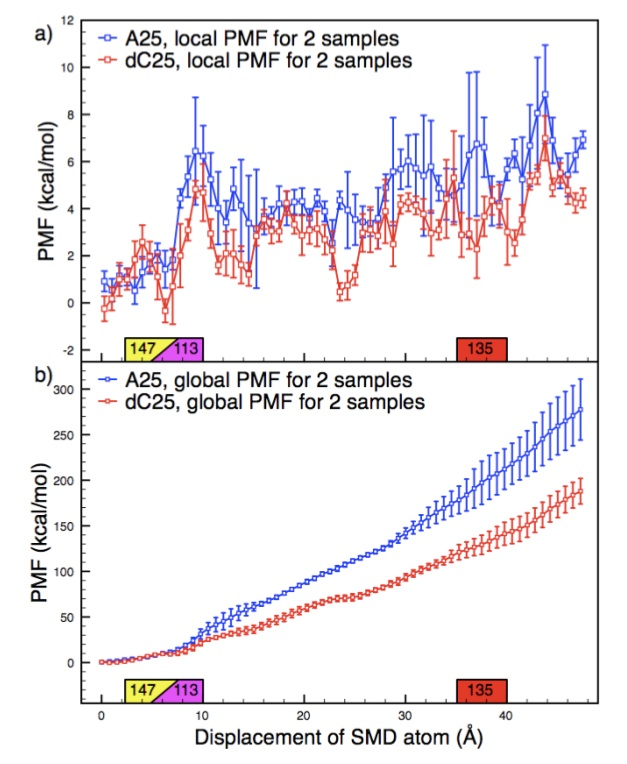
\includegraphics[width=4.0in]{full_trans_1every3_b}
%  \end{center}
%  \caption{Figure from JCTC Publication, where a) Local free energy profiles of \atf and \dctf translocation from the top of the constriction to the bottom of the $trans$-entrance; each profile was derived from two samples. Labeled along the $x$-axis are protein residues Met-147, Lys-113, and Leu-135.  The residue labels span 5~{\AA} from when the pulled atom to first phosphate atom passes the labeled residue. The plot shows poor separation of \atf and \dctf when considering the error bars, though a general trend where \atf has a higher free energy profile than \dctf is observed. An overall increase in the free energy profile is observed from left to right, which is expected as more residues enter the confining dimensions of the constriction and transmembrane barrel. b) Global free energy profile of \atf and \dctf translocation from the top of the constriction to the bottom of the trans-entrance; each profile was derived from two samples. The plot shows good discrimination of \atf and \dctf beyond the error bars. The error bars indicate greater sample-to-sample variation around the constriction and towards the end of the transmembrane barrel, which may indicate non-steric contributions at these points.}
%  \label{full_trans_local}
%\end{figure}

  \begin{figure}[!h]
  \begin{center}
    \subfigure{\label{fig:fulltrans-a}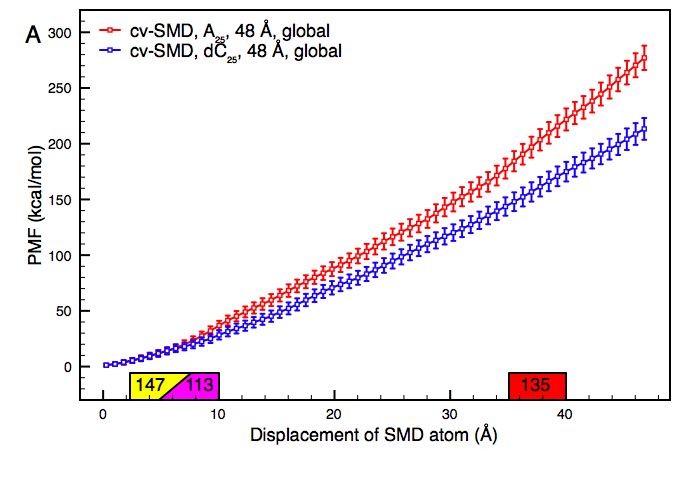
\includegraphics[width=4.0in]{full_trans_16sample_cv-SMD_A25_vs_dC25_nice_adjusted}}
    \subfigure{\label{fig:fulltrans-b}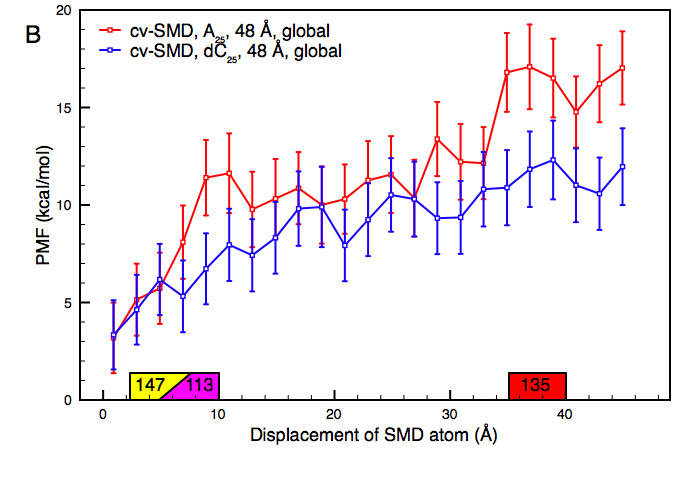
\includegraphics[width=4.0in]{full_trans_16sample_cv-SMD_A25_vs_dC25_local_nice_adjusted}}  
    \end{center}
    \caption[Local and global free energy profiles of \atf and \dctf translocation from the top of the constriction to the bottom of the $trans$-entrance of wild type \ahl]{Local and global free energy profiles of \atf and \dctf translocation from the top of the constriction to the bottom of the $trans$-entrance of wild type \ahlnsp. A) Global free energy profile of \atf and \dctf
translocation; each profile was derived from 16 samples, calculated using a bin width of 0.75~{\AA}. Labelled along the $x$-axis are protein residues Met-147, Lys-113, and Leu-135. The residue labels span 5~{\AA} from when the pulled atom to first
phosphate atom passes the labelled residue. The free energy estimate for \atf is $\sim$30\% higher than that of \dctf at the end of the 48~{\AA} reaction coordinate. The plots show discrimination of \atf and \dctf beyond the error bars after 11~{\AA} of translocation. The gradients of both profiles gradually increase, which is in line with expectations that pulling additional nucleotides into the confining dimensions of the transmembrane barrel raises the energetic barriers to further translocation. B) Local free energy profiles of \atf and \dctf translocation; each profile was derived from 16 samples, calculated using a bin width of 2~{\AA}. For these systems, the local environments lead to consistently higher energetic barriers to translocation for \atfnsp. The \atf profiles also exhibits larger peaks than \dctfnsp, most notably at 9~{\AA} and 37~{\AA}.}
  \label{full_trans_local}
\end{figure}

% The high-level scientific objective for this project is to compute free energy profiles of the translocation process of DNA along the vertical axis of a transmembrane protein pore buried in a lipid membrane bilayer. This is a project that has been ongoing for nearly three years % (which was initiated before my transition to LSU),
% and has consumed a total of about 6M SUs so far.

The work that has been published so far covers relatively low sampled instances of nucleotide and single nucleotide translocation through wild type and mutated protein pores, yielding good results and has established the groundwork for further publications. The project uses the parallel MD code NAMD and as also led to a grid-enabled version of NAMD developed by us to perform steered MD simulations including the capability to connect to distributed haptic devices. This work is currently funded by the UK's EPSRC (equivalent to the US NSF).

Using the TRAC grant that was awarded to us last year, we have significantly improved the sampling of these results, plus additional results. For the latest set of data, each profile is calculated from 16 samples (instead of 2-4 samples), which has greatly improved the quality and reliability of the data. Systems \dctfnsp-WT,  \dconsp-WT, \atfnsp-WT,  \aonsp-WT,  and \dctfnsp-Mut (see Table~\ref{table:systems1}), were included in the JCTC publication with a low number of samples and now stand at 16 samples each. Systems \dconsp-Mut, \atfnsp-Mut, and \aonsp-Mut, were not previously explored and now have full 16 sample data-sets. Using these data-sets we have been able to make conclusions such as the negligible impact of the nucleotide base sterics, and are able to point to nucleotide base stacking as  one of the causes for the experimentally observed difference between poly(A) and poly(dC) translocation times.

Additionally, over the last year we have used the molecular models established in the cv-SMD simulations to test the system using an alternative translocation method. The method we examined was Adaptive Biasing Force (ABF). Here the translocating atom (and thus the attached molecule) is moved with a biasing force, which acts to overcome energy barriers in order to translocate along a reaction coordinate. The biasing force adapts to the free energy landscape on-the-fly, calculating the free energy and biasing force based on the forces acting on the atom in question, and applying the force directly to that atom. In this way, ABF surpasses the need for certain approximations to be made related to the use of Jarzynski's Equality and the requirement of a stiff cv-SMD harmonic spring, allowing us to assess the impact that these approximations had on the cv-SMD data. Furthermore, ABF does not constrain the biased atom in axes orthogonal to the reaction coordinate, allowing enhanced sampling of the reaction coordinate. So far, we have examined key ABF simulation parameters to allow for the exploration of the \ahl-nucleotide systems, and have produced single sample free energy profiles for \atfnsp-ABF and \dctfnsp-ABF (see Table~\ref{table:systems1}).



\begin{table}[!h]
\begin{center}
  \caption{The translocation molecules and pore types to be simulated. `Wild Type' indicates \ahl with no mutated residues; 'Mutant' indicates \ahl mutant L147M.\newline }
\label{table:systems1}
\begin{tabular}{| c | c | c | c | c | c |}
\hline
Pulling & System & \ahl Type & Nucleotide & Nucleotides & Samples \\
Method & Name &  & Base &  & Performed \\
\hline
cv-SMD & \aonsp-WT & Wild Type & Adenine & 1 & 16/16  \\
cv-SMD & \atfnsp-WT & Wild Type & Adenine & 25 & 16/16  \\
cv-SMD & \dconsp-WT & Wild Type & Deoxycytosine & 1 & 16/16  \\
cv-SMD & \dctfnsp-WT & Wild Type & Deoxycytosine & 25 & 16/16 \\
cv-SMD & \aonsp-Mut & Mutant & Adenine & 1 & 16/16  \\
cv-SMD & \atfnsp-Mut & Mutant & Adenine & 25 & 16/16  \\
cv-SMD & \dconsp-Mut & Mutant & Deoxycytosine & 1 & 16/16  \\
cv-SMD & \dctfnsp-Mut & Mutant & Deoxycytosine & 25 & 16/16  \\
ABF & \atfnsp-ABF & Wild Type & Adenine & 25 & 1  \\
ABF & \dctfnsp-ABF & Wild Type & Deoxycytosine & 25 & 1  \\
\hline
\end{tabular}
\end{center}
\end{table}

% Current and near-future work, also forms the basis of a joint US-UK submission to the NSF (in collaboration with Prof.'s Zuzanna Siwy (UC-Irvine) and Stefan Howorka (London)).

%\jhanote{Shantenu to liase with Peter and Hugh on the next phase, including ABF} 

%In the next phase of the project, we aim to expand the sampling of all the explored systems %to yield solid and consistent results. The published set of data represents 2 to 6 samples per %free energy profile, we are now looking to expand this to 16 samples for each system %investigated (see Table~\ref{table:systems}). This will allow us to confidently compare the %results to means of translocation other than cv-SMD. 


We have ascertained that to allow for the production of quality data that may be compared to our cv-SMD results, we require multi-sample (at least 4) data-sets of systems  \atfnsp-ABF-$\zeta$5k, \dctfnsp-ABF-$\zeta$5k,  \aonsp-ABF-$\zeta$5k,  and \dconsp-ABF-$\zeta$5k (see Table~\ref{table:systems2}). For these simulations, there is a key ABF parameter, $\zeta$, that dictates how many timesteps the biased atom is required to exist within the boundaries of a particular bin along the reaction coordinate before the biasing force in applied. This parameter influences the impact of non-equilibrium effects, the average speed of translocation, plus the computational cost, and its optimum value is highly sensitive to the size and flexibility of the translocating molecule. Therefore, we will also be performing simulations where the $\zeta$ value is pushed to more computationally intensive limits to determine its full impact on the data quality. These systems are \atfnsp-ABF-$\zeta$20k, \dctfnsp-ABF-$\zeta$20k,  \atfnsp-ABF-$\zeta$80k, \dctfnsp-ABF-$\zeta$80k, as listed in Table~\ref{table:systems2}.


\begin{table}[!h]
\begin{center}
  \caption{The translocation molecules and pore types to be simulated. `Wild Type' indicates \ahl with no mutated residues; 'Mutant' indicates \ahl mutant L147M.\newline }
\label{table:systems2}
\begin{tabular}{| c | c | c | c | c | c |}
\hline
Pulling & System & \ahl Type & Nucleotide & Nucleotides & Samples \\
Method & Name &  & Base &  & Performed \\
\hline
ABF & \atfnsp-ABF-$\zeta$5k & Wild Type & Adenine & 25 & 4  \\
ABF & \atfnsp-ABF-$\zeta$20k & Wild Type & Adenine & 25 & 4  \\
ABF & \atfnsp-ABF-$\zeta$80k & Wild Type & Adenine & 25 & 2  \\
ABF & \dctfnsp-ABF-$\zeta$5k & Wild Type & Deoxycytosine & 25 & 4  \\
ABF & \dctfnsp-ABF-$\zeta$20k & Wild Type & Deoxycytosine & 25 & 4  \\
ABF & \dctfnsp-ABF-$\zeta$80k & Wild Type & Deoxycytosine & 25 & 2 \\
ABF & \aonsp-ABF-$\zeta$5k & Wild Type & Adenine & 1 & 4  \\
ABF & \dconsp-ABF-$\zeta$5k & Wild Type & Deoxycytosine & 1 & 4  \\
\hline
\end{tabular}
\end{center}
\end{table}

For systems of this size (approximately 325000 atoms) and for the timescales of interest, it is necessary to use a HPC parallel MD Engine, such as NAMD.  We use NAMD on either 128 or 256 processors typically. We have used Ranger and QueenBee extensively for earlier simulations for this project. Our simulations of cv-SMD sampling has so far consumed about 4.25M SUs (to be contrasted with 6.75M for the overall project) and about 0.75M SUs more are required to finish sampling the remaining systems (specifically, multi-sampled ABF simulations).  Therefore we ask for  0.75M to be allocated to us for use on this project.


\section*{Project 2: Computational Study of non-coding Functional RNAs: Binding mechanism of Riboswitches}


\jhanote{Joohyun -- Please start updating}
%Increasing attention has focused on targeting RNAs for drug design~\cite{foloppe}. 

While increasing evidence indicates a critical role of structured nc-RNAs in gene regulations of both transcription and translation levels, suggesting the potential of targeting RNA for drug design~\cite{foloppe} and bioengineering applications, an understanding of the interactions of nc-RNAs with other molecules such as small metabolite, proteins, and RNAs remains as fundamental challenges.  The roles of computational means, therefore, are critical component for holistic understanding on dynamics and interactions of RNAs.

Among nc-RNAs, our primary targets are riboswitch RNAs. Riboswitches are regulatory RNAs that control the expression of downstream genes. Small metabolite molecules, such as amino acids, nucleotides, coenzymes etc., can bind to riboswitches as effectors in vivo~\cite{mandal}.  In our recent research efforts, the S-box riboswitch (also called SAM-I riboswitch), one member of the riboswitch family that regulates genes related to the metabolism of sulfur and methionine, has been extensively investigated with atomistic simulations.  This riboswitch choose alternative conformation depending on binding of a SAM .  When S-adenosylmethionine (SAM) is bound, the aptamer domain forms anti-anti-terminator (AAT) conformation, which turns off the downstream genes by forming the terminator (T). Otherwise, the anti-terminator (AT) is formed prohibiting the T element formation for continuing transcription process (Figure 3a)~\cite{brooke}. Although the structure of the s-box in the anti-anti-terminator (AAT) conformation has been solved via X-ray crystallography, it is just a static view of how SAM binds to the s-box.  Using extensive all-atom simulations, we became to propose a novel binding mechanism of the SAM-I riboswitch with a SAM in which the role of entropic barrier for the AAT formation as well as the role of $Mg^2+$ specifically bound in the tertiary core structure.  We reported our simulation results in recent conferences and the paper of obtained results were recently submitted to the journal, Nucleic Acids Research.  The paper is now under the review.~\cite{SAM-I-NAR2009} Continuing our efforts, the goal of this study is to probe the dynamic interactions between the s-box riboswitch and SAM at the nanoscale and to explore determinants for the specificity. In particular, we aim to extend our main strategy, combining MD and statistical analysis, for i) other constructs of SAM-I that differ from each other in potentially different secondary structures and tertiary interactions, ii) different sequences in SAM-I family, and iii) other SAM riboswiches (SAM-II and SAM-III) for which X-ray structures were recently reported.  To estimate binding affinity, we employed the Molecular Mechanics - Poisson Boltzmann Surface Area (MM-PBSA) approach and expect to develop novel theoretical developments because of the challenges arising from strong electrostatic interactions involved.  Sampling is a also very important task and for that purpose, replica exchange molecular dynamics (REMD) protocol is attempted.  Our recent development for the distributed adaptive REMD, that is described below, will help us to carry out simulations for these sizable systems.

Also, related experiments are carried out in collaboration with Prof. Fareed Aboul-ela (who has several funded projects -- both Federally and Regional for experiments in collaboration with our simulations). Since a significant advantage of atomistic simulation is the ability to be able to explore details that are typically inaccessible to experiments; while at the same time providing the opportunity for our simulation results will be validated using biochemical and biophysical experiments.

\begin{figure}
\begin{center}
  \subfigure[]{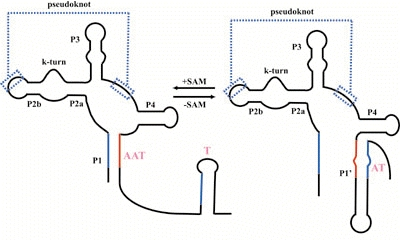
\includegraphics[scale=0.60]{ss-schema}} \hspace{0.05in}
  \subfigure[]{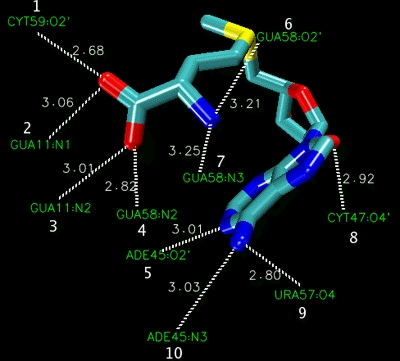
\includegraphics[scale=0.40]{ligand-atom2}}
\end{center}
\caption{(a) Schematic of the secondary structures of s-box riboswitch with SAM bound (left; in the AAT state) and without SAM 
(right; in the AT state), (b) predicted ligand-SAM interactions with s-box}
\end{figure}


\begin{figure}
\begin{center}
  \subfigure[]{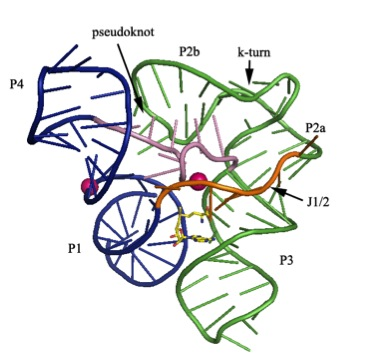
\includegraphics[scale=0.33]{sbox_3D}}
  \subfigure[]{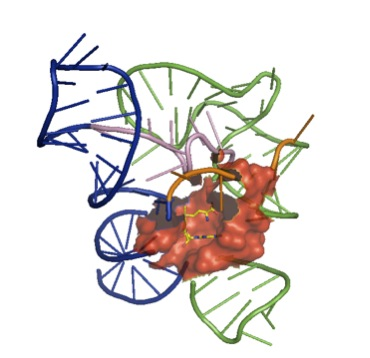
\includegraphics[scale=0.33]{binding_pocket-2}}
  \subfigure[]{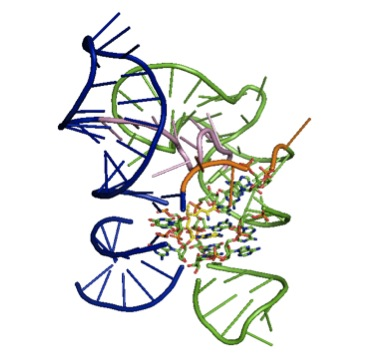
\includegraphics[scale=0.33]{binding_pocket-1}}
\end{center}
\caption{(i) The structure of the S-box riboswitch; (ii) S-box with SAM bound; (iii) Residue number: 7, 11, 
12, 45-47, 57-59, 88, 89}
\end{figure}


\subsubsection*{Initial Results}

Here, we brief MD simulation protocols used for the long time MD simulations of the SAM-I riboswitch and new findings reported in the paper~\cite{SAM-I-NAR2009}.  The starting point of all simulations is the X-ray crystal structure of SAM binding to the AAT conformation of s-box riboswitch (PDB: 2GIS)~\cite{montange}. In the simulation of the SAM free s-box riboswitch, SAM is directly removed from the x-ray crystal structure and replaced with solvent water. The amber99bsc0 correction force field is used here~\cite{alberto}. Parameters for SAM are from the Generalized Amber Force Field (GAFF) and missing parameters are calculated using ANTECHAMBER~\cite{wang}. Positions of added hydrogens are guessed using PSFGEN within NAMD 2.6. Then the RNA molecules are solvated in a cubic solvent box of TIP3P waters with a 16A padding in all directions. Sodium and magnesium ions are distributed around the RNA molecules and neutralize charge of the system. The total number of atoms in the system is 56,000. Energy minimizations are carried out on all of the systems to remove bad contacts. Starting from 0 K, the temperature is raised 10 K for every 10,000 steps and is held constant after reaching the desired temperature (310 K) using temperature reassignment. MD simulations are performed in the NPT ensemble with the pressure maintained using the Langevin piston method with a period of 100 fs and decay times of 50 fs. The time step is 2fs for both equilibration and production phase. Bond lengths between hydrogens and heavy atoms are constrained using SHAKE. The long-range electrostatics is treated with the Particle Mesh Ewald (PME) method with a cutoff distance 12A.  All MD simulations are carried out by using a parallel version of NAMD 2.6.  VMD, wordom~\cite{moe} and homemade scripts are employed to analyze the trajectories. All snapshots of structural images are made using VMD.

%All simulations are performed using NAMD 2.6 on LSU (Tezpur) and LONI (Queenbee) Linux clusters. 

\begin{figure}
\begin{center}
   \subfigure[]{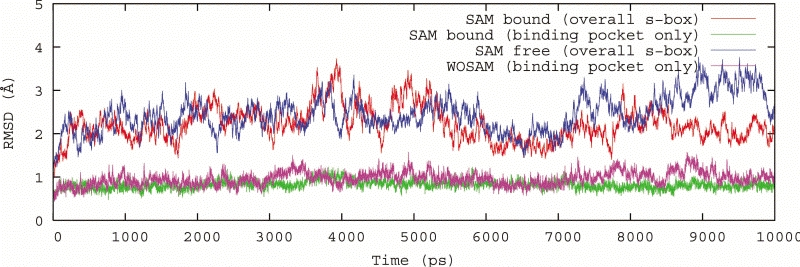
\includegraphics[scale=0.42]{rmsd}} \newline
   \subfigure[]{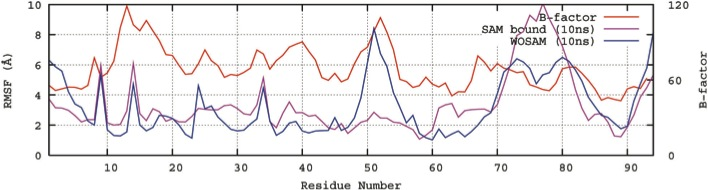
\includegraphics[scale=0.49]{RMSD_residue}}
\end{center}
\caption{RMSD of overall s-box and binding pocket only in SAM bound and WOSAM (short for the 
trajectory of SAM free s-box riboswitch) trajectories  with reference to the crystal structure; (b) Root mean square fluctuation (RMSF) and B-factor of each residue of s-box riboswitch from MD trajectories}
\end{figure}

\begin{figure}
\begin{center}
   \subfigure[]{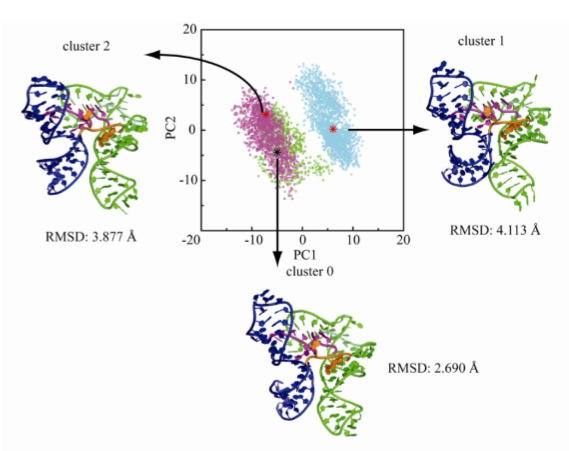
\includegraphics[scale=0.45]{cluster_2D}}
   \subfigure[]{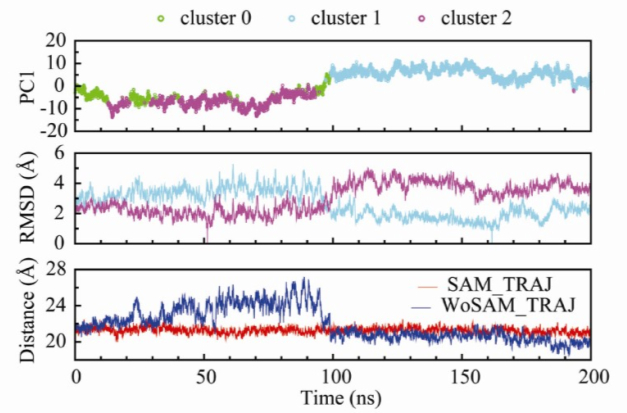
\includegraphics[scale=0.35]{cluster_1D}} \end{center} \caption{Clustering and Principal Component Analysis (PCA) point towards a chopstick-like motion involving P1 and P3 helices in the absence of SAM.  (a) Projections of snapshots of the SAM free trajectory are plotted against the first two principal components and color coded according to a k=3 k-means clustering: cluster 0: magenta, cluster 1, green, cluster 2, magenta. Representative snapshots from each cluster are also shown. This plot indicates that snapshots can be broadly clustered into two groups (cluster 1 and cluster 3) with cluster 2 representing a group with characteristics similar to those of cluster 3. The projection along PC1 broadly separates the clusters, while projection along PC2 completes the separation between clusters 1 and 3. Structures of representative snapshots indicate that clusters are distinguished by a dramatic change in relative position of P1 and P3. (b) From top to bottom: The time evolution of the first principle component of the SAM free trajectory. RMSD for each snapshot in the SAM free relative to the representative snapshots for cluster 1 (cyan curve) and for cluster 3 (magenta curve). The distance between the Center of Mass (COM) of P1 and P3 for the SAM free trajectory (blue) and for the SAM bound trajectory (red).  During the first half of the SAM free trajectory, P1 and P3 helices move apart (clusters 0 and 2), then they move back together during the second half of the trajectory (cluster 1).}

\end{figure}

Our initial achievements are illustrated in Figure 5 and Figure 6.  Our results suggest that the presence of SAM in the binding pocket is critical to form P1 helix overcoming the entropic cost for bringing two distal strands in proximity.  The essential dynamics found with the SAM-free trajectory are shown in Figure 6 with clustering results, indicating the characteristic long time dynamics in the SAM-free system. 

To estimate the binding affinity, we chose MM-PBSA and according to our results, strong electrostatic interactions between SAM and SAM-I as well as the importance of inner-shell bound $Mg^{2+}$ binding are well noticed as critical components for the overall SAM binding mechanism.  

\begin{figure}
\begin{center}
  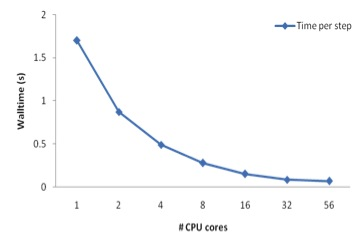
\includegraphics[scale=0.660]{56k_scaling-2} \caption{Wall-clock times taken (in second) for each step at different processor counts. The measurement was done with Queen Bee }
\end{center}
\end{figure}

\begin{table}[h]
\begin{center}
  \caption{Riboswitch simulations and expected computing resources. Note that the estimated SUs for MM-PBSA calculation is about the additional MD simulation with the SAM-free RNA system \jhanote{Please update} }
\label{table:systems}
\begin{tabular}{| c | c | c | c |}
\hline
Molecular System & Type of Calculation &   Method or Package  &   SUs required \\
\hline
SAM-I & MD &  NAMD &  30K\\
SAM-I & MM-PBSA & NAMD & 30K \\
SAM-I & PCA/Clustering &  AMBER and scripts &  50K\\
SAM-II &MD &  NAMD &  15K\\
SAM-II & MM-PBSA & NAMD & 15K \\
SAM-II & PCA/Clustering & AMBER and scripts & 50K \\
SAM-II & REMD &  NAMD &  450K\\
SAM-III &MD &  NAMD &  30K\\
SAM-III & MM-PBSA & NAMD & 30K \\
SAM-III & PCA/Clustering & AMBER and scripts & 50K \\
\hline
\end{tabular}
\end{center}
\end{table}

\subsubsection*{Requested Computational Resources}

We estimated the total computational time based on our simple benchmark and the benchmark found in the TeraGrid web site as mentioned above.  In Figure 7, we show the scaling performance with MD simulation package such as NAMD.  The benchmark was done with Queen Bee.  When using 32 cores, the time taken per step is approximately 0.06s; thus the wall clock time required to complete 1ns is .34 day; in other words for a 56K system, 1 ns simulations require $\approx$ 300 CPU hours.  Thus each 100 ns simulation requires approximately 30,000 CPU hrs.  Based on this estimation, in Table 2, expected CPU costs are estimated.  We expect 750,000 SUs are needed for this project and considering similar performance between Ranger and Kraken, (also assuming Queen Bee's performance close to Abe. See {\url{http://staging.teragrid.org/userinfo/aus/namd_benchmark.php}} ) 500,000 SUs are requested with Ranger and the remaining 250,000 SUs are requested with Kraken, respectively.


\section*{Project 3: UCL Contribution}


\section*{Project 4: Expeditions in Distributed Computing using SAGA}


\jhanote{Yaakoub-- Please take a first shot. Include resource request for LINCOLN. Please also update
with some details of the TG10 paper submission.}

Advances in Grid applications have simply not kept pace with advances in other aspects of distributed CyberInfrastructure, such as Grid middleware -- whether measured by the number of existing applications that can easily utilize the many advanced features offered by distributed infrastructure or measured by the number of novel applications capable of using the infrastructure. A key impediment in the accelerated development and deployment of Grid applications is the scarcity of high-level application programming abstractions that bridge the divide between the needs of Grid applications and the capabilities offered by middleware.  Much Grid development has focused on the support for legacy parallel and cluster application codes as a way of ensuring scientific relevance.  The benefit of the Grid paradigm, however, will come from new application development that does not depend on the homogeneous and relatively static model of resource performance inherited from parallel or cluster legacies.  % The lack of such application-level programming abstractions is compounded by the fact that there exist incompatible and often changing Grid middleware systems in both research and production environments.

To address these challenges and in particular to find a solution to the universal, apparently intractable problem of successfully Grid-enabling applications, several applications groups expressed the desire for a simple programmatic interface that is widely-adopted, usable and available.  The goal of such an interface would be to provide a ``grid counterpart to MPI'' (at least in impact if not in details) and that would supply developers with a simple, uniform, and standard programmatic interface with which to develop distributed applications.  Thanks to the efforts of many contributors, but in particular the PI's group, an initial specification of such a ``grid counterpart to MPI'' now exists -- the Simple API for Grid Applications (SAGA)~\cite{saga_url}. As of early 2008, SAGA is now an Open Grid Forum (OGF) technical recommendation.

\subsubsection*{Developing and Deploying Applications using SAGA}

A wide range of applications have been developed using SAGA -- ranging from regular compute intensive applications but involving multiple resources ~\cite{saga_escience07, gmac, REMD-PhilTranA2009}, applications with multiple components and possibly irregular runtime requirements~\cite{saga_loosely_coupled, teragrid08} as well data-intensive applications ~\cite{saga_data_intensive, saga_grid_cloud} using programming abstractions such as MapReduce~\footnote{Implementation of MapReduce using SAGA is funded by Google} An initial prototype of a ``general pilot-job'' framework using SAGA that can be utilized for Replica-Exchange that enables the {\it trivial} utilisation of multiple distributed resources across TeraGrid has been developed. This is currently work in progress, but we anticipate sufficient progress to begin testing the framework using our 56K riboswitch model.~\cite{REMD-PhilTranA2009}. A Brief schematic of Distributed Adaptive Replica Exchange Molecular Dynamics is shown in Figure 8.  Our current framework implements the Generalized Pilot-Job feature with the BigJob abstraction built upon SAGA and utilization of the framework is the key component for successful massive REMD simulations for our project on riboswitch studies.

\begin{figure} \begin{center} 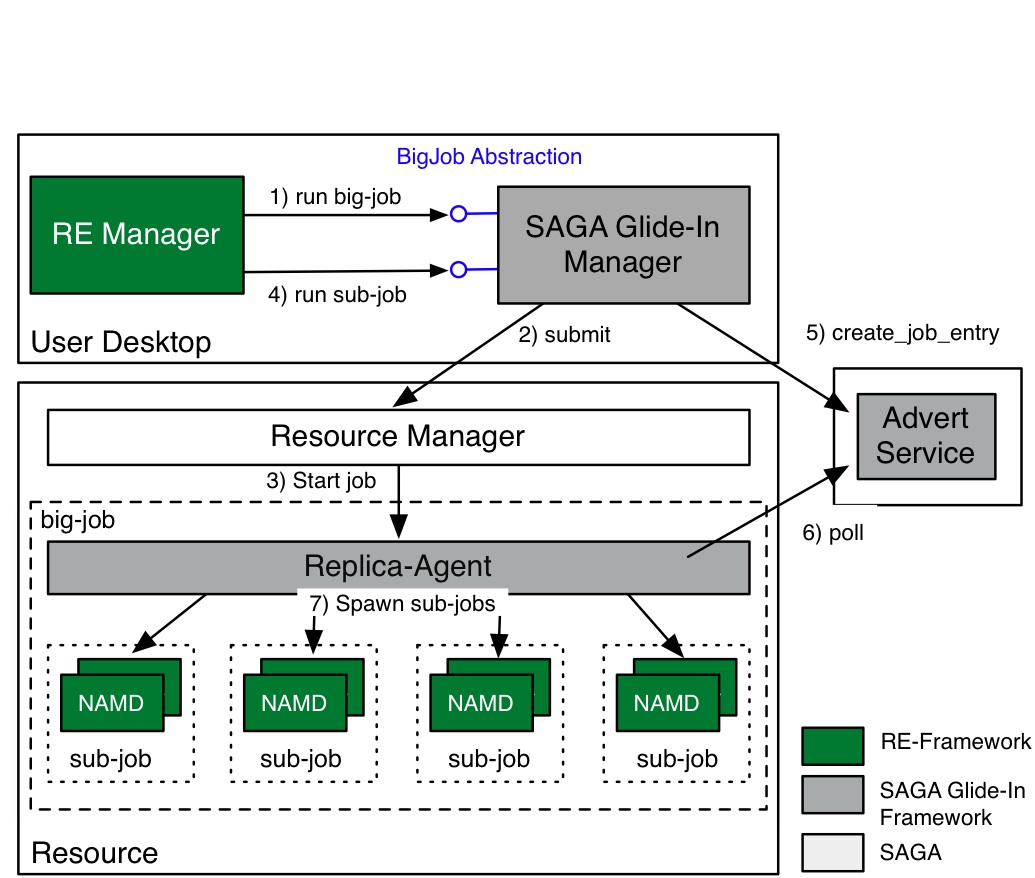
\includegraphics[scale=0.55]{DARE-MD} \end{center} \caption{Schematic of Distributed Adaptive Replica Exchange framework using the BigJob abstraction that is built upon SAGA. It is proposed that DARE-MD framework will ultimately become part of the GridChem Science Gateway (in which the PI and co-PI Kim are involved).} \label{fig:results} \end{figure}

\subsubsection*{Developing Autonomic Computing Frameworks for CO$_2$ Sequestration Studies using SAGA}

Global energy needs today present serious challenges: the increasing demand for energy must be met, however at the same time the emissions of greenhouse gases into the atmosphere must be reduced. Even as alternative energy sources continue to develop and gain popularity, the fact remains that fossil carbon resources will continue to be in heavy use (in both developing and industrialized countries) and consequently generate large volumes of carbon dioxide ~\cite{GeoRPT}. The atmospheric impact of this greenhouse gas can be abated through capturing and sequestering significant fractions of the produced CO$_2$.

For long-term storage of large volumes of CO$_2$, porous subsurface geologic formations are ideal candidates: these are the same formations responsible for the existence of oil and gas reservoirs. Indeed much the technology behind carbon dioxide sequestration (including drilling, gas injection, reservoir management and of course reservoir simulation) stems from drilling, petroleum and reservoir engineering. Injecting CO$_2$ into an oil-gas reservoir can also lead to improved oil recovery by ``pushing out'' the oil and gas for production, this allows for reduced net cost through increased revenues from oil and gas production ~\cite{EORBook}.

\begin{figure}
\begin{center}
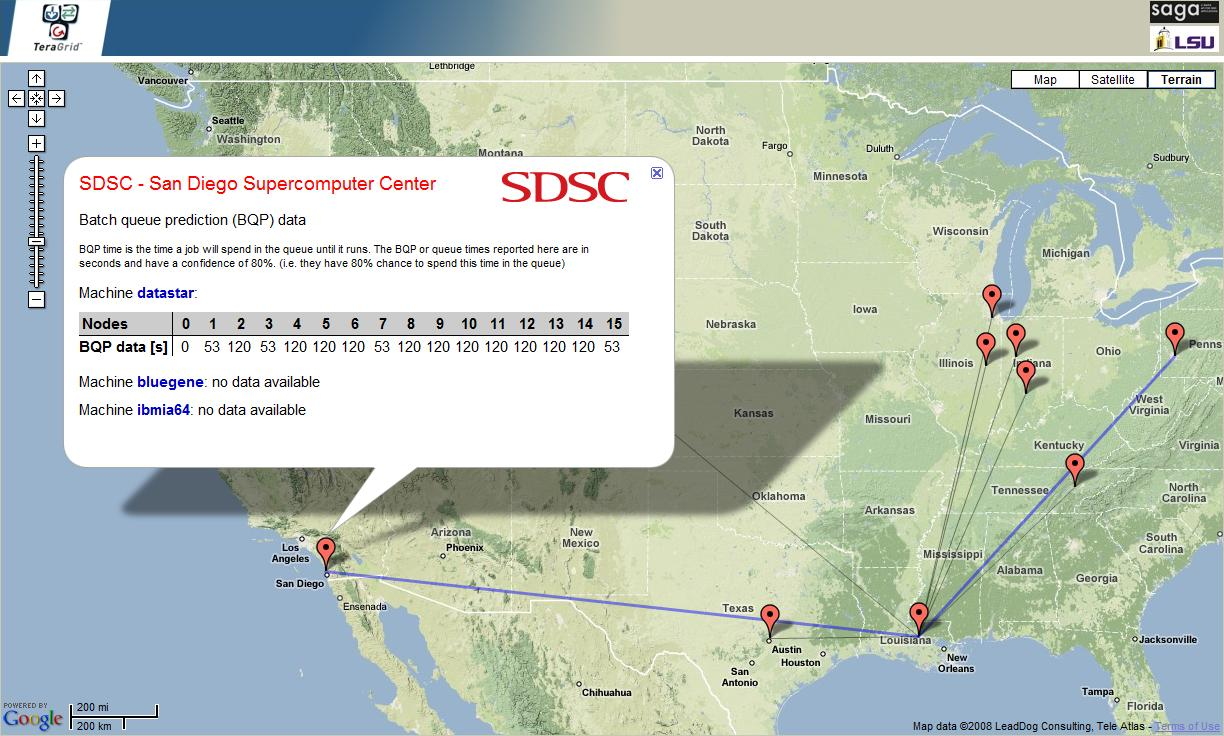
\includegraphics[scale=0.33]{gmaps_bqp.jpg}
\end{center}
\caption{A snapshot of an application using batch-queue-prediction system to dynamically determine the best resource to spawn a sub-task to; the noteworthy point is that the entire decision process is at the application level -- the fact that the application has to spawn a job of requirements X is mapped to a resource requirements, BQP is used to determine the resource based upon optimal availability and then the application uses SAGA to spawn and launch the sub-task onto the chose resource. A paper demonstrating this feature working across the TeraGrid won the Performance Challenge Award at TeraGrid 2008 (Ref.~\cite{teragrid08})}
\label{}
\end{figure}

One of the major areas of research in this field is the characterization of reservoirs that are safe and secure, environmentally and geologically and are therefore promising candidates for CO$_2$ sequestration ~\cite{GeoRPT,Luigi}. Our efforts are directed towards developing CyberInfrastructure tools, technologies and abstractions that facilitate large scale reservoir characterization and forecasting studies.

Since the amount of information obtained directly from reservoirs is very small compared to the actual size of the reservoir, history matching techniques have been developed to match actual reservoir production with simulated reservoir production, therefore obtaining a more ``satisfactory'' set of reservoir models. One of the promising approaches to history matching is the use of Ensemble Kalman filters (EnKF) ~\cite{KalmanPaper, DO2007, LiEnKF07, DO2006}.

\begin{table}[!h]
\begin{center}
 \caption{Summary of allocation usage for a typical reservoir study}
\begin{tabular}{| c | c |}
\hline
SU cost per simulation for history matching& 240 SUs \\ 
\hline
SU cost per simulation for forecast & 320 SUs \\ 
\hline
Number of simulations (ensemble members) & 200 simulations \\ 
\hline
Total Cost in SUs & 112k SUs\\
\hline
\end{tabular}
\end{center}
\end{table}

Ensemble Kalman filters are recursive filters that can be used to handle large, noisy data; the data in this case would be the results and parameters from ensembles of reservoir models that are sent through the filter to obtain the ``true state'' of the data. Since the reservoir model varies from one ensemble to another, the run-time characteristics of the ensemble simulation are irregular and hard to predict. Furthermore, at simulation times when real historical data is available, all the data from the different ensembles at that simulation time must be compared to the actual production data, before the simulations are allowed to proceed. This translates into a global synchronization point for all ensembles; hence performing large scale studies for complex reservoirs in a reasonable amount of time would benefit greatly from the use of distributed, high performance, high throughput and on-demand computing resources.

\begin{figure}
\begin{center}
\includegraphics*[scale=0.4,angle=0]{3StageKalmanFilter}
\end{center}
\caption{Schematic illustrating the variability between stages of a typical
  ensemble Kalman filter based simulation. The end-to-end
  application consists of several stages; in general at each stage the
  number of models generated varies in size and duration. From References~\cite{teragrid08, gmac}}
\label{fig:irregular_execution}
\end{figure}

To this end we developed several components: a CO$_2$ sequestration simulator and an autonomic, self-monitoring, self healing and self optimizing job management framework: the Lazarus framework ~\cite{gmac}. Early investigation of the single machine performance of Lazarus and {\it Scale-Out} performance on multiple distributed TeraGrid resources are promising, with a significantly reduced total time to completion in the optimized, distributed cases.

\begin{figure}
\begin{center}
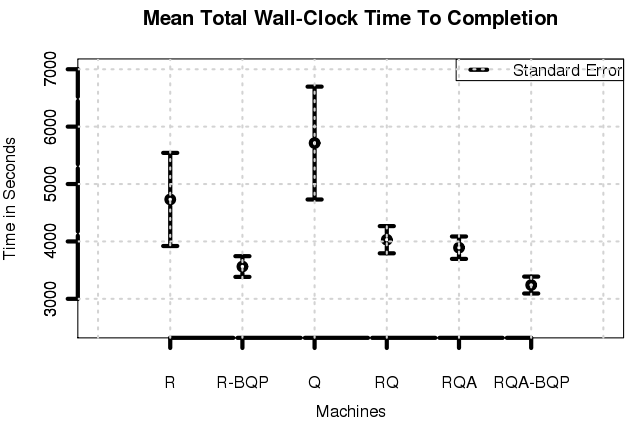
\includegraphics[scale=0.8]{Figure7.png}
\end{center}
\caption{Demonstrating the effectiveness of Distributed Applications Developed  Using SAGA to Scale-Out. From Left to Right, Performance as measured by the time-to-completeness of a well-defined workload when using: (i) Ranger only (ii) Ranger (with BQP service) only, (iii) QueenBee only, (iii) Ranger and QueenBee, (iv) Ranger, QueenBee and Abe concurrently (v) Ranger, QueenBee 
  and Abe when using BQP service. From Ref.~\cite{gmac} }
\label{fig:results}
\end{figure}

\subsubsection*{Utilizing Application-level Interoperability across TeraGrid and DEISA}
As part of NSF funded HPCOPS Award, LONI has begun a year long project to utilize the aggregated computational power of the Federated Grids of DEISA and TeraGrid. The aim of the project is to (i) work towards an integrated infrastructure that supports application level-interoperability and, (ii) having created the infrastructure, apply it to the dual challenge of understanding the conformational changes and determining the free energy of biological systems. Specifically, the high-level aim of this project is to enable scientific applications to utilise the federated capabilities of the TeraGrid, DEISA and LONI systems, to enhance the understanding of HIV-1 enzymes and epidermal growth factor receptors (EGFR) implicated in lung cancer -- important science drivers in general. The aim of this project is to use several Replica-based and Replica-Exchange simulations for HIV-1 \& EGFR research, on multiple TeraGrid, LONI and DEISA resources, working concurrently towards the solution of a single problem instance -- the rapid computation of free-energies of binding with high-levels precision.

{\it Resource Requirements:} For Project 3, we require 750,000 SUs. This in turn is divided into a component for the Interoperability Project (500K) and the EnKF-based Sequestration Project (250K). The latter is, a somewhat more experimental component of this proposal, where we do not have clear estimates and benchmarking data. However, based upon our experience/publications alluded to in the previous paragraph, each "experiment" that we conduct, (i.e. application that we develop), requires a minimum of 50000 SUs. For example, running a reservoir simulation for a simulation time of two weeks (typical period of historical production data gathering) consumes roughly ten minutes on four cores.  With two hundred ensembles (typical number of ensembles), running for a simulation time of fifteen years will consume 48k SUs. This obviously is the medium range of simulations; a more detailed reservoir model will naturally consume more SUs per simulation, multiplied by a large number of ensembles and the SUs required to perform the history matching increases dramatically. To complete the forecast stage, we will need to run the same ensembles for an extended period of time (reservoir depletion/workover, enhanced oil recovery and CO$_2$ sequestration) which roughly would range between twenty to thirty years in simulation time, that is an additional 64k-96k SUs, placing the total in the range of 112k-144k SUs for a single complete reservoir study.

The TeraGrid-DEISA Interoperability project -- built upon validated and ready to run models, has already acquired significant resources (several million CPU hours) on DEISA machines; our request for 500K is to support initial production runs of the VPH (Virtual Physiological Human) models and test the infrastructure for Scale-Out tests -- intra-TeraGrid as well as TeraGrid-DEISA Grids, performed on the VPH Models.

\section*{Summary}
% In summary, our request is for 1.25M SUs bound (non-roaming) to Ranger, 0.75M SUs bound to Kraken and a 750K roaming allocation over QB-ABE/Ranger/Kraken.  To state the obvious, if a primary aim of our work is to investigate the ability of distributed applications to {\it Scale-Out}, then it is imperative that there be an underlying resource allocation to support the work. We aim to develop frameworks such as Lazarus and Faust to support the ability of applications to {\it Scale-Out} in a manner that is independent of the specifics of the applications.  By extension, in order to scale-out to the TeraGrid and DEISA combined resources (one of the motivations for interoperability), we will also have to scale-out on the TeraGrid.  In general, there are instances where we have chosen to request non-roaming allocations but request more than one machine for the same project; this is to hedge against lengthy, but more challengingly, variable queue length (load) factors. However, the bulk of our resource request is non-roaming ($\approx$ 75\%).

\begin{table}[!h]
\begin{center}
  \caption{Resource distribution requests for different projects \jhanote{This will need revision and updating} \newline}
\label{table:systems}
\begin{tabular}{|c| c | c | c | }
\hline 
Project & Resource & Total Request & Roaming \\
\hline
I & Ranger  & 750K & Non-Roaming \\
I & Kraken &  500K  & Non-Roaming \\
\hline
II & Ranger & 500K & Non Roaming \\
II & Kraken & 250k & Non-Roaming \\
\hline
IIIa & Abe-QB/Kraken/Ranger & 250K & Roaming \\
IIIb & Abe-QB/Kraken/Ranger & 500K & Roaming \\
\hline
\end{tabular}
\end{center}
\end{table}

\section*{Supporting Grants}
\jhanote{Shantenu to update. (i) ExTECNI, (ii) BIPAS and others.} The PI leads Work Package 4 of the NSF Funded Cybertools Project (http://www.cybertools.org) (NSF Award Number-00000, Total Value \$12M).  PI-Jha is also the co-PI of LSU/LONI's HPCOPS NSF award, ``Joining the TeraGrid'', member of the Scientific Board of the LONI Institute.  Project 2 is funded by multiple Louisiana Board of Regents award and an LSU Faculty Award (PI Jha). Integration of SAGA with applications is part of Cybertools and the PI also holds multiple peer-reviewed awards for the development and integration of SAGA.  The Interoperability Project~\cite{interop_url} is currently funded by an NSF HPCOPS award, and is being executed by the PI (Jha). See PI's vitae for full grant listing. Part of EnKF work is funded by the UCoMS project, Department of Energy and Louisiana Board of Regents award No. DE-FG02- 04ER46136

\section*{TeraGrid User Support} Since our applications have been developed, tested and benchmarked on the TeraGrid resources we are requesting allocations on, we do not foresee any need for support from TeraGrid personnel. However, as part of the TeraGrid-DEISA Interoperability, it is probable we will submit a supplemental request for ASTA support (in Q4 of 2009).

\bibliographystyle{unsrt}
\bibliography{jha_loni_alloc_jul01}

\end{document}

